\documentclass{article}

\usepackage[utf8]{inputenc}

% Packages
\usepackage{amsmath,amssymb}
\usepackage{bm}% boldmath
\usepackage{listings} % Code block (source code) \begin{lstlisting} 
\usepackage{natbib}
\usepackage{graphicx}
\usepackage{lmodern}
\usepackage[usenames,dvipsnames,svgnames,table]{xcolor}
\usepackage[textwidth=16cm,textheight=23cm]{geometry}

%\usepackage{inconsolata} % New monospace font

% URL
\usepackage{url}
\usepackage[colorlinks=true, a4paper=true, pdfstartview=FitV, linkcolor=blue, citecolor=blue, urlcolor=blue]{hyperref}

% Figures
\usepackage[font=small, labelfont=bf]{caption}
\usepackage{subfig} % Subfigures. Uses \subfloat[captions text]{figure}

% Tables
\usepackage{booktabs}   % Allows the use of \toprule, \midrule and \bottomrule in tables for horizontal lines
\newcommand{\ra}[1]{\renewcommand{\arraystretch}{#1}} % spaces in tables

% Itemize
\usepackage{enumitem}

% Commands
%\newcommand{\code}[1]{\texttt{#1}} % \code{inline code}
\newcommand{\code}[1]{{\small\ttfamily #1}} % \code{inline code}
\newcommand{\expval}[1]{\langle #1 \rangle} %
\renewcommand{\theequation}{\arabic{section}.\arabic{equation}} % Book format equation
\renewcommand{\thefigure}{\arabic{section}.\arabic{figure}} % Book format figure
\renewcommand{\vec}[1]{{\bf #1}} % Lars likes this better than arrow

% Set page attribution
\setlength{\parindent}{0pt}


% PSTRICKS
\usepackage{pstricks,pst-node,pst-tree} % includes graph additions
\usepackage{pst-pdf} % Compiles the pictures
\usepackage{pst-node}
\usepackage{pst-plot}
\usepackage{pst-3dplot}
%\usepackage{pstricks-add,babel}




\lstset{
language=Python,                        % Code langugage
commentstyle=\color{gray},              % Comments font
basicstyle=\small\ttfamily,             % Code font, Examples: \footnotesize, \ttfamily
keywordstyle=\bfseries\color{blue},
stringstyle=\color{orange},
numbers=left,                           % Line nums position
numberstyle=\tiny,                      % Line-numbers fonts
stepnumber=1,                           % Step between two line-numbers
numbersep=5pt,                          % How far are line-numbers from code
frame=none,                             % A frame around the code
tabsize=4,                              % Default tab size
captionpos=b,                           % Caption-position = bottom
breaklines=true,                        % Automatic line breaking?
breakatwhitespace=false,                % Automatic breaks only at whitespace?
showspaces=false,                       % Dont make spaces visible
showstringspaces=false,                 % Dont make spaces visible in strings
showtabs=false,                         % Dont make tabls visible
belowskip=8pt,
morekeywords={range, xrange},
% backgroundcolor=\color{yellow}
% emph={[2]root,base}
% morekeywords={one,two,three,four,five,six,seven,eight,
}


%commentstyle=\color{gray},              % Comments font
%basicstyle=\small,                      % Code font, Examples: \footnotesize, \ttfamily



%basicstyle=\footnotesize\ttfamily,
%keywordstyle=\bfseries\color{green!40!black},
%commentstyle=\itshape\color{purple!40!black},
%identifierstyle=\color{blue},
%stringstyle=\color{orange},







% ***************************************************
% HEADER INFORMATION

\title{Exercise 4}
\author{Molecular Statistics, Week 4}
\date{2014}

% ***************************************************

\begin{document}


% ***************************************************
% BEGIN DOCUMENT
% ***************************************************

\maketitle

\section{Introduction}

The goals of this exercise:
\begin{enumerate}
    \item Extend your MD-program to three dimension using the supplied module.

    \item Implement a 3D Velo-Verlet solver.

    \item Extend your program with functions to calculate the following properties:
    \begin{enumerate}
        \item Kinetic energy
        \item Total energy
        \item Temperature
        \item Pressure
    \end{enumerate}

    \item Visualize your results in a video.

\end{enumerate}


% Is there a numpy handout?
You should read the Numpy handout available on the course website.


\subsection{Lennard-Jones potential and periodic boundary conditions}

The potential we are using this week is almost the same Lennard-Jones potential
as we saw last week.  You may recall from your simulation last week, that the
calculation of the particle pair-interactions took a long time to compute, even
with only 10-20 particles.
To speed up the calculation time we can make the approximation that only
particles closer than a certain minimum distance $r_{\mathrm{cut}}$ are
interacting.
This is a justified approximation, since particles that are
far apart have weak interactions.
Here we set $r_{\mathrm{cut}} = 2.5$.
Using this approximation, we can define the the potential energy between two
interacting particles $i$ and $j$ by:

%\begin{eqnarray}
%    U_{ij} &=& 4 \epsilon \left[ \left(\frac{\sigma}{r_{ij}} \right)^{12} - \left(\frac{\sigma}{r_{ij}} \right)^6 \right] -E_{\mathrm{cut}} \ \ \mathrm{if}\ \ r_{ij} < r_{\mathrm{cut}}\\
%    U_{ij} &=& 0 \ \ \mathrm{if}\ \ r_{ij} \ge  r_{\mathrm{cut}}
%\end{eqnarray}

%\begin{eqnarray}
%    U_{ij} &= 
%    \begin{cases}
%        \ \ 4 \epsilon \left[ \left(\frac{\sigma}{r_{ij}} \right)^{12} - \left(\frac{\sigma}{r_{ij}} \right)^6 \right] -E_{\mathrm{cut}} & \mathrm{if}\ \ r_{ij} < r_{\mathrm{cut}}\\
%        \ \ 0 & \mathrm{if}\ \ r_{ij} \ge  r_{\mathrm{cut}}
%    \end{cases}
%\end{eqnarray}
\begin{eqnarray}
    U_{ij} &= 
    \begin{cases}
        \ \ 4 \left[ \left(\frac{1}{r_{ij}} \right)^{12} - \left(\frac{1}{r_{ij}} \right)^6 \right] -E_{\mathrm{cut}} & \mathrm{if}\ \ r_{ij} < r_{\mathrm{cut}}\\
        \ \ 0 & \mathrm{if}\ \ r_{ij} \ge  r_{\mathrm{cut}}
    \end{cases}
\end{eqnarray}

The derivatives of the potential energy are used to calculate the forces
between particles:

\begin{equation}
    \mathbf{F} = -\nabla U =
    -\left(
        \frac{\partial U}{\partial x_1},\
        \frac{\partial U}{\partial y_1},\
        \frac{\partial U}{\partial z_1},\
        \frac{\partial U}{\partial x_2},\
        \frac{\partial U}{\partial y_2},\
        \frac{\partial U}{\partial z_2},\
        \ldots\ ,
        \frac{\partial U}{\partial x_n},\
        \frac{\partial U}{\partial y_n},\
        \frac{\partial U}{\partial z_n}
    \right)
\end{equation}

The $x$-components of the force between two interacting particles $i$ and $j$
are:

%\begin{eqnarray}
%-\frac{\partial}{\partial x_i} U_{ij}&=& -48\ \frac{x_j - x_i}{r^2_{ij}}\left[ \left(\frac{1}{r_{ij}} \right)^{12} - 0.5 \left(\frac{1}{r_{ij}} \right)^6 \right]\ \ \mathrm{if}\ \ r_{ij} < r_{\mathrm{cut}}\\
%-\frac{\partial}{\partial x_i} U_{ij} &=& 0\ \ \mathrm{if}\ \ r_{ij} \ge  r_{\mathrm{cut}}\\
%-\frac{\partial}{\partial x_j} U_{ij} &=& 48\ \frac{x_j - x_i}{r^2_{ij}}\left[ \left(\frac{1}{r_{ij}} \right)^{12} - 0.5 \left(\frac{1}{r_{ij}} \right)^6 \right]\ \ \mathrm{if}\ \ r_{ij} < r_{\mathrm{cut}}\\
%-\frac{\partial}{\partial x_j} U_{ij} &=& 0\ \ \mathrm{if}\ \ r_{ij} \ge  r_{\mathrm{cut}}
%\end{eqnarray}

\begin{eqnarray}
    -\frac{\partial}{\partial x_i} U_{ij}&=& 
    \begin{cases}
        \ \ -48\ \frac{x_j - x_i}{r^2_{ij}}
        \left[ \left(\frac{1}{r_{ij}} \right)^{12} - 0.5 \left(\frac{1}{r_{ij}} \right)^6 \right]
        & \mathrm{if}\ \ r_{ij} < r_{\mathrm{cut}} \\
        \ \ 0 & \mathrm{if}\ \ r_{ij} \ge  r_{\mathrm{cut}}
    \end{cases}\label{eq:force_i}\\
    -\frac{\partial}{\partial x_j} U_{ij}&=&
    \begin{cases}
        \ \ \ \ 48\ \frac{x_j - x_i}{r^2_{ij}}
        \left[ \left(\frac{1}{r_{ij}} \right)^{12} - 0.5 \left(\frac{1}{r_{ij}} \right)^6 \right]
        & \mathrm{if}\ \ r_{ij} < r_{\mathrm{cut}} \\
        \ \ 0 & \mathrm{if}\ \ r_{ij} \ge  r_{\mathrm{cut}}
    \end{cases}\label{eq:force_j}
\end{eqnarray}

The $y$- and $z$-components are of course similar.

\subsection{Velo-Verlet integration and periodic boundary conditions}

Last week your setup confined the particles in the simulation inside a box with
hard walls. Today's exercise uses periodic boundary conditions in the
minimum-image convention.
% Jan's notes?
You don't have to implement this code, since it's already implemented in the FORTRAN library you
will be using. The Velo-Verlet integrator you have to implement is thus very
simple (and identical to last week).
The Velo-Verlet equations for integrating the positions and velocities are (in
the $x$-direction for one particle):

\begin{eqnarray}
x(t + dt) &=& x(t) + dt\ v_x(t) + 0.5\ dt^2\ a_x(t)\label{eq:position_x}\\
v_x(t + dt) &=& v_x(t) + 0.5\ dt \left[a_x(t) + a_x(t+dt)\right]\label{eq:speed_x}
\end{eqnarray}

In the program you will be implementing today, we will again set the mass of the particles
to 1, such that the value of the acceleration is equal to the value of the force.\\

Let's recap: The Velo-Verlet algorithm uses the forces, velocities and
positions from the current position to calculate the forces, velocities and
positions after the next time-step. In short it is a three-step procedure:

\begin{enumerate}
    \item Calculate new positions using Eq. \ref{eq:position_x}
    \item Calculate new forces using Eq. \ref{eq:force_i}-\ref{eq:force_j}
    \item Calculate new velocities using Eq. \ref{eq:speed_x}
\end{enumerate}

The resulting forces, velocities and particle positions are then saved as input
for the next Velo-Verlet integration step.

\subsection{Kinetic energy}

The total kinetic energy of the system can be calculated as:

\begin{equation}
    E_{\mathrm{kin}} = \sum_i \frac{1}{2} m_i |\vec{v_i}|^2
\end{equation}

In our simulation $m_i$ is set to 1, so the above reduces to:

\begin{equation}
    E_{\mathrm{kin}} = \frac{1}{2} \sum_i |\vec{v_i}| \cdot |\vec{v_i}|
\end{equation}

\textbf{Hint:} If you do this in Numpy, the above summation is simply carried
out as (something like):

\begin{lstlisting}[language=python]
e_kin = np.sum(V * V) * 0.5
\end{lstlisting}

% V = Vx + Vy + Vz. Something they've seen in lectures?
Why is this true? What does V * V do and what does np.sum() do?

\subsection{Conservation of energy}

If your simulation is successful the total energy will be conserved. That is:

\begin{equation}
    E_{\mathrm{total}} = E_{\mathrm{pot}} + E_{\mathrm{kin}} \approx \mathrm{constant}
\end{equation}

Conservation of energy can sometimes fail during a MD simulation. Often this
is due to the timestep $dt$ being too large, which causes the numerical
Velo-Verlet integration to fail.

\subsection{Instantaneous temperature}

The first thermodynamic property we will derive from our simulation is the instantaneous temperature,
that is the temperature as a function of time, $T(t)$.
You will sometimes see the temperature defined in terms of the average kinetic energy \textit{per} degree of freedom in a system:

\begin{eqnarray}
    \langle E_{\alpha} \rangle = \frac{1}{2} k_\mathrm{B} \ T
\end{eqnarray}

where $\alpha$ denotes the degrees of freedom in the system. The above states that each degree of freedom gives a contribution to the temperature which is proportional to the kinetic energy of the individual particles.\\
Instead of this formulation it is more practical for our purpose to write the temperature in its instantaneous form:

\begin{eqnarray}
    T(t) &=& 2 \frac{\langle E_{\alpha}(t) \rangle}{k_\mathrm{B} \ N_\alpha }\\
         &=& \sum_i \frac{m_i|\vec{v_i}| \cdot |\vec{v_i}|}{k_\mathrm{B} \ N_\alpha}
\end{eqnarray}

where $N_\alpha$ is the number of degrees of freedoms, i.e.~$N_\alpha = N_{\mathrm{dimensions}} \cdot N_{\mathrm{particles}}$. Notice, that we use fundamental units and simple masses, so $k_\mathrm{B} = 1$ and $m_i = 1$.\\\\

\textbf{Hint:} If you do this in Numpy, this can be written easily as:
\begin{lstlisting}[language=python]
temperature = 2.0 * e_kin / np.size(V)

# or

temperature = np.mean(V * V)
\end{lstlisting}

Why this is true? What does np.size() calculate? What does np.mean() calculate?
Why do both implementations the yield the same result?

\subsection{Instantaneous Pressure}

The instantaneous pressure in a Van der Waal gas simulation can be calculated
as:

\begin{eqnarray}
    P(t) & = & \rho \ T(t) + \frac{1}{3V_\mathrm{box}}  \sum_{i>j} \vec{F_{ij}} \cdot \vec{r_{ij}}\\
         & = & \rho \ T(t) + \frac{1}{3V_\mathrm{box}} W_{vir} \label{eq:intmp}
\end{eqnarray}

where $V_\mathrm{box}$ is the volume of the box, $\rho$ is the particle-density
of the box  and $W_{vir} = \sum_{i>j} \vec{F_{ij}} \cdot \vec{r_{ij}}$ is the
Clausius virial function (or \textit{virial} for short) of the system.\\

Since we were not using a standard Lennard-Jones potential (we use a small
cut-off distance), we have to add a small correction (the \textit{tail
correction}) to Eq. \ref{eq:intmp} in order to account for the interaction we are
neglecting:

\begin{eqnarray}
    \Delta P_\mathrm{tail} & = & \frac{16}{3}\pi \rho \left[ \frac{2}{3}\left( \frac{\sigma}{r_{\mathrm{cut}}} \right)^9 - \left(\frac{\sigma}{r_{\mathrm{cut}}} \right)^3 \right]
\end{eqnarray}

Here we simply set $\sigma = 1$. Remember
$r_{\mathrm{cut}} = 2.5$.

\newpage

\section{Numpy Exercises}

% TODO generelt
% copy.copy(V) <-- earliere week?

% TODO methods
% np.save
% np.load
% random, random.seed, random.randint

% TODO Vector methods
% restrictions (no append method)
% min, max (maybe argmin and argmax?)
% sum, prod
% mean
% shape
% +=, -=, *=, /=

% Start with numpy exercises to make sure students understand how it works, rather than the MD part?

When working with Python "in the real world" you will most often use Numerical
Python (NumPy) and vectorization.
This is because it is faster and easier.
Firstly we'll import the module \code{numpy}.


\begin{lstlisting}[language=python]
import numpy as np
\end{lstlisting}

Numpy is a fast library of functions and data types.
It is mostly used for substituting the normal Python List for a new data type
called \code{ndarray}.

As an example, generating an empty list of zeros with the two different methods:

\begin{lstlisting}
list = [0.0 for i in range(5)] # Normal list
array = np.zeros(5)           # Numpy array
\end{lstlisting}

% Haven't touched upon += etc. so far, so skip? Or introduce?
A huge advantage of using Numpy arrays is vectorization commands.
%You can change a variable by using commands like
%"\code{+=}",
%"\code{-=}",
%"\code{*=}",
%"\code{/=}". So the code
%
%\begin{lstlisting}
%a = 45
%a = a + 5
%\end{lstlisting}
%
%is equivalent too
%
%\begin{lstlisting}
%a = 45
%a += 5
%\end{lstlisting}
%
%\begin{enumerate}
%    \setcounter{enumi}{1}
%    \item Execute and evaluate the above command. What does it do?
%\end{enumerate}

You can perform mathematical operations on every element at once in a Numpy array, just like you would on a single element. E.g. 
\begin{lstlisting}
V = np.zeros(5)
%V += 5
V = V + 5
\end{lstlisting}

This however doesn't work with normal Python Lists.

\begin{enumerate}
    \setcounter{enumi}{1}
    \item Execute and evaluate the above command. What is the result of V?
\end{enumerate}

{\bf Note:}
When you create a Numpy array, you always specify a size.
This also represents how much computer memory is allocated by Numpy.
For this reason it is not possible to use the \code{append} method, as with
the normal Python list.\\

If you are not sure how big your array is going to be, you can create a list, append elements,
and then after all elements are appended, convert it too a Numpy array as following.

\begin{lstlisting}
L = []
for i in range(10):
    L.append(i)
L = np.array(L)
\end{lstlisting}

% Whole part seems out of place and a bit trivial
%A very useful command to use is the \code{np.arange()}, which is similar to the range().
%
%\begin{enumerate}
%    \setcounter{enumi}{3}
%    \item Execute the code
%
%\begin{lstlisting}
%num_vector = np.arange(0, 5)
%print num_vector
%num_vector = np.arange(0, 5, 0.1)
%print num_vector
%\end{lstlisting}
%
%    and explain what the method \code{np.arange()} does.
%
%
%    \item What does \code{np.sum()} do and what is the result of the follow code?
%
%\begin{lstlisting}
%np.sum(num_vector)
%\end{lstlisting}
%
%    Answer: 122.5
%
%    \item What does \code{np.mean()} do and what is the result of the follow code?
%
%\begin{lstlisting}
%np.mean(num_vector)
%\end{lstlisting}
%
%    Answer: 2.45
%
%    \item What is the value of \code{np.pi}.
%
%    \item What does \code{np.random.uniform(0.0, 1.0)} do?
%
%    \item (Optional) How to get a random float from a normal distribution,
%        using Numpy? Create a list of 1000 random numbers and plot the
%        distribution using Pylab.
%
%        {\em Hint:} Use Google.
%
%\end{enumerate}

\newpage

\section{Molecular Dynamics simulation}

Before you start this weeks exercise, please make you you have downloaded the
material from the course website.\\

% TODO REWRITE THE FOLLOWING TO MATCH MATERIAL
Before you start, download the two files from absalon, \code{md\_header.py} and
\code{forces.so}. Put both files in the same folder as the Python program you are
working on today. \code{md\_header.py} contains functions to initialize the particles,
calculate the Lennard-Jones forces and energy as well as a function to
visualize a 3D video of your simulation. \code{forces.so} implements the
calculation of the Lennard-Jones forces in a very efficient FORTRAN routine. You
don't have to worry about the technical details of this, just know that the
FORTRAN routine is about 300 times faster than the same code running in Python.

Make a new Python program, and name it \code{exercise\_4.py}.
In the first two lines import Numpy and the three functions from the downloaded
module.

\begin{lstlisting}
import numpy as np
import md_header as md
import video3d
\end{lstlisting}

Last week you wrote your own code to initialize the particle positions,
velocities, box\_width etc. The initialize\_particles() function you
imported is a bit more advanced.
The new initialize\_particles() function takes as arguments the number of
particles, the given temperature and a desired particle density.\\

The temperature option is used to scale the particle velocities appropriately
(see section 1.5) and the rho keyword is used to scale the width of the box
according to the number of particles (we need to be able to specify a particle
density in order to calculate the pressure correctly, see section 1.6)

\begin{enumerate}

    \item Initialize your system with the following code:

\begin{lstlisting}
R, V, F, box_width = initialize_particles(n_particles, temperature, rho)
\end{lstlisting}

        Suggested values are temperature = 2.0 and rho = 0.1.
        Don't worry you will get a chance to play around with these values later

\end{enumerate}

You will notice that initialize\_particles() returns four values.
\code{R} is the coordinate matrix. It is an Nx3 matrix, which holds for each of N particles
the X, Y and Z coordinates.
Likewise \code{V} and \code{F} holds the initial velocities and forces, respectively.
\code{box\_width} is the width of the scaled box, which today you cannot specify this yourself,
because it is based on the density of the particles.\\

Now it's time to test the initialize\_particles function.


\begin{enumerate}
    \setcounter{enumi}{1}

    \item What comes out of \code{initialize\_particles(n\_particles,
        temperature, rho)} if you set \code{n\_particles = 10}, \code{temperature = 2.0} and
        \code{rho = 0.1}? What do \code{R}, \code{V} and \code{F} contain? Can
        you explain why?

\end{enumerate}

The second new function you got from the md module is \code{lennard\_jones()} - which
can be used like this:

\begin{lstlisting}[language=python]
e_pot, F, w_vir = lennard_jones(R, box_width)
\end{lstlisting}

\code{lennard\_jones} takes as arguments the position matrix \code{R} and \code{box\_width}.
Just like last week, the \code{lennard\_jones} function returns the potential energy
\code{e\_pot}, a force matrix \code{F}, but now also the virial of the system,
\code{w\_vir} (see section 1.6).\\


\begin{enumerate}
    \setcounter{enumi}{2}

    \item
    Now it's time to test the \code{lennard\_jones} function. Instead of giving R as input
    to lennard\_jones, call the function with the following \code{R\_test} matrix:

\begin{lstlisting}
R_test = np.array([[0.7, 2.3, 0.7], [0.7,  0.7, 2.3], [0.7, 0.7, 0.7]])
\end{lstlisting}

    and \code{box\_width = 3.10}. That is:

\begin{lstlisting}
print lennard_jones(R_tests, 3.10)
\end{lstlisting}

    The potential energy is -0.635, the virial -3.732. The forces matrix (rounded
    values):

\begin{lstlisting}
array([[-1.16   1.24  -0.09]
        [-1.16  -0.09   1.24]
        [ 0.0    0.0    0.  ]])
\end{lstlisting}

    The $z$-components of the force are correctly 0 (why?).

\end{enumerate}

Now it is time to implement the Velo-Verlet solver from last week, but using
the new module and Numpy.

\begin{enumerate}
    \setcounter{enumi}{3}

    \item Somewhere in your program file put the solver code in:

\begin{lstlisting}
for n in range(n_steps):
    # Step 1: Calculate new positions
    R = R + ...

    # Step 2: Calculate new forces
    F_old = copy.copy(F)
    e_pot, F, w_vir = lennard_jones(R, box_width)

    #Step 3: Calculate new Velocities:
    V = V + ...
\end{lstlisting}

    {\bf Hint:} Look at the last exercise if you need inspiration on where to
    put the solver code.

    \item Initialize your system with 40 particles, \code{rho = 1.1} and
        \code{temperature = 2.0.}
        Run your simulation for 1000 steps with $dt = 0.001$.
        Every 10 steps print the potential energy. The potential energy should
        stabilize around -20 if your solver works properly.

    \item Now would be a good time to implement the video function.
        The new 3D video is used like the other by adding frames like;

\begin{lstlisting}
# Add Frame
video3d.add_frame(R)

# Save movie
video3d.save(box_width, 'my_video')

\end{lstlisting}

        And add frame every 10'th step in the Velo-Verlet step.

    \item Run 500 steps and save a video.

\end{enumerate}


You have now successfully implemented an MD simulation of a Lennard-Jones gas.
The goal now is to use the equations from section 1 to calculate interesting
physical properties of your system.

\begin{enumerate}
    \setcounter{enumi}{7}

    \item Use the equations from section 1.3 to calculate the kinetic energy.
        Print the kinetic energy, potential energy and total energy each 10
        step.

    \item Make three empty lists called Ekin\_list, Epot\_list and Etot\_list.
        Append

\begin{lstlisting}[language=python]
Ekin_list = []
Epot_list = []
Etot_list = []

for n in range(n_steps):

    """ Your Velo-Verlet solver code
        is here ...
    """

if (n % 10):
    # Calculate e_kin and e_tot
    # here!

    Ekin_list.append(e_kin)
    Epot_list.append(e_pot)
    Etot_list.append(e_tot)
\end{lstlisting}

    \item Run your simulation for 10,000 steps. Do not save a video, since this
        will take several minutes to compile. Use Pylab to make a plot of the
        energies vs. time.:

\begin{lstlisting}
pylab.clf()
pylab.plot(Ekin_list, 'r-', label='Kinetic Energy')
pylab.plot(Epot_list, 'b-', label='Potential Energy')
pylab.plot(Etot_list, 'g-', label='Total Energy')
pylab.legend() # Plot labels in figure
pylab.savefig("my_energy.png")
\end{lstlisting}

    How does the energies evolve if you run your simulation with 40 particles at T =
    2.0? Now run your simulation at a lower temperature (maybe T = 0.5). How does
    the energy change ?

    \begin{figure}[h!]
        \begin{center}
            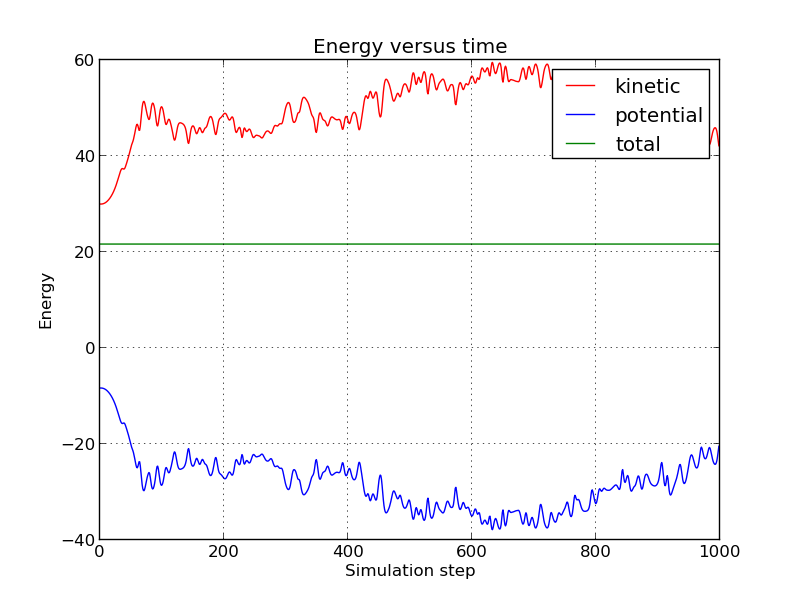
\includegraphics[width=0.75\textwidth]{energy.png}
            \caption{
                Evolution of energies during an MD simulation with
                temperature = 0.5, 40 particles, rho = 0.1, for 10,000 steps
                and saving every 10'th step.
            }
            \label{fig:energies}
        \end{center}
    \end{figure}


    \item Use the equations from section 1.5 to calculate the instantaneous
    temperatures during the simulation. 

    \item Like in the previous question, make an empty list called T\_list and
    append the current temperature every 10 steps. Use Pylab to make a plot of
    this list. See Figure \ref{fig:temperature} for example.

    \begin{figure}[h!]
        \begin{center}
            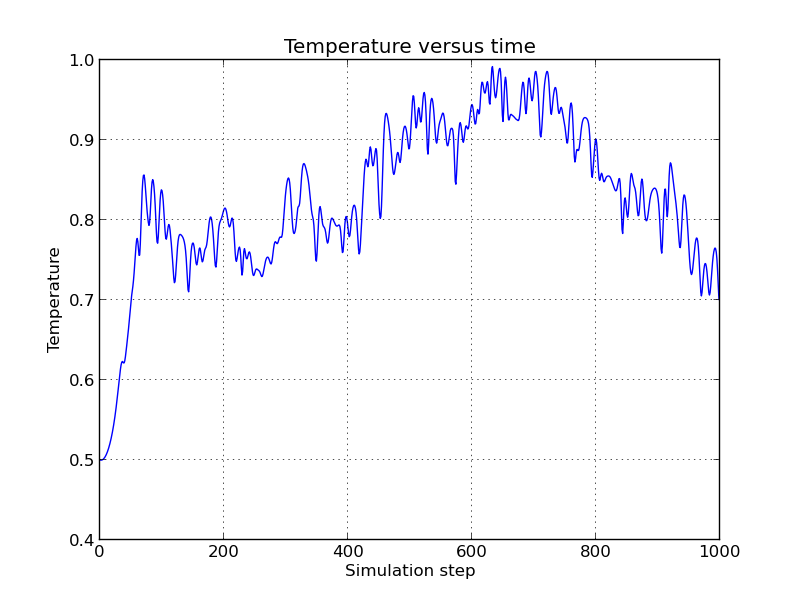
\includegraphics[width=0.75\textwidth]{temperature.png}
            \caption{Evolution of temperature during an MD simulation with T = 0.5, 40 particles, rho = 0.1.}
            \label{fig:temperature}
        \end{center}
    \end{figure}

    Does the temperature you calculate correspond to the temperature you
    specified when you initialized your particles? Run your simulation at T =
    0.05. What could easily go wrong now?

    \item Answer this question before you proceed: Why is the gas a Van der
        Waals gas and not an ideal gas? I.e. why isn't the pressure simply $p =
        \frac{N T}{V}$.

    Use the equations from section 1.6 to calculate the instantaneous pressure during the simulation. 

    \item Use Pylab to plot the pressure during the simulation, as done in the
        previous exercises. How does the temperature and particle density
        affect the pressure? See Figure \ref{fig:pressure} for example.

    \begin{figure}[h!]
        \begin{center}
            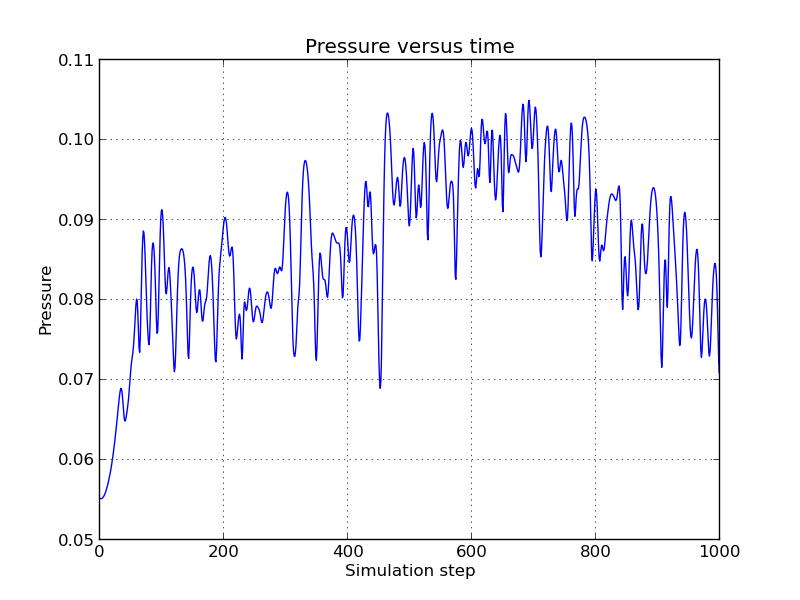
\includegraphics[width=0.75\textwidth]{pressure.png}
            \caption{Evolution of pressure during an MD simulation with T = 0.5, 40 particles, rho = 0.1.}
            \label{fig:pressure}
        \end{center}
    \end{figure}

\end{enumerate}

% ***************************************************
% END DOCUMENT
% ***************************************************

\end{document}
